\chapter{입자, 파동, 그리고 분해능에 필요한 에너지}

\section{입자인가, 장인가?}

입자물리학은 무엇을 다루는가? 입자---그러나 이 대답은 곧바로 오래된 질문을 불러온다. 자연은 불연속적인가? 여기서 불연속적이라는 말은 물질이 서로 분리된, 더는 나눌 수 없는 단위들로 이루어져 있다는 뜻이지, 빈틈없이 재치 있다는 뜻이 아니다. 그리스어 \emph{아토모스}는 나눌 수 없다는 뜻이지만, 오늘날 원자라고 부르는 물체는 쪼갤 수 있다. 일단 \emph{입자}를 불연속적인 단위를 가리키는 일반적인 이름으로 쓰겠다.

이와 대립하는 그림은 연속체이다. 이 그림에서 물질은 서로 분리된 조각들의 집합이 아니라 공간에 연속적으로 퍼져 있는 것이다. 이를 표현하는 자연스러운 언어는 장의 언어이다. 장은 위치의 함수이다. 물질의 밀도는 장이며, 전기장과 자기장도 장이다. 전기장과 자기장은 하전 입자의 운동을 결정하지만, 장 자체는 고전적으로 공간에 연속적으로 분포한다고 여긴다.

이러한 생각이 역사적으로 등장한 순서를 지나치게 엄밀하게 따질 필요는 없다. 이 순서는 신뢰할 만한 연대기를 제공하기 때문이 아니라 논증의 논리를 보여 주기 때문에 유용하다. 입자 어휘에는 원자, 분자, 충돌, 국소화된 물체가 포함되고, 연속체 어휘에는 장과 연속적으로 변하는 물리량이 포함된다. 어느 그림이 옳을까? 양자역학은 어느 쪽도 완전히 옳을 수 없게 하지만, 어느 쪽도 완전히 틀릴 수 없게 한다.

이 논의는 어느 정도 자체적으로 이해할 수 있도록 전개되지만, 뒤의 논증에서는 양자역학, 고전역학, 특수상대성이론, 전자기학을 활용한다. 당장 던질 질문은 더 단순하다. 물질이 실제로 불연속적이라고 사람들이 처음 확신하게 된 계기는 무엇이었을까?

\section{불연속적인 물질을 뒷받침하는 화학적 증거}

적어도 여기서 논리적으로 구성한 설명에 따르면, 최초의 유력한 증거는 물리학이 아니라 화학에서 나왔다. 이 구분은 인위적이다. 화학은 대체로 원자와 분자의 물리학이기 때문이다. 돌턴은 서로 다른 물질에서 같은 수의 분자가 차지하는 질량을 비교했다. 시료에 같은 수의 분자가 들어 있음을 확인하는 일 자체가 큰 문제였다. 여기서 아보가드로의 이름이 등장하며, 1몰은 아보가드로 수만큼의 분자를 뜻한다. 분자 수가 같은 시료들을 비교하는 데에는 그 수의 실제 값이 필요하지 않았다.

눈에 띄는 규칙성은 몰질량이 수소의 몰질량을 단위로 삼았을 때 대략 정수배가 된다는 것이었다. 그 배수는 대체로 \(3/2\), \(\pi\) 또는 임의의 실수가 아니라 정수에 가까운 수였다. 예를 들어 탄소12는 수소가 나타내는 질량 단위의 대략 열두 배에 해당한다. 이는 물질이 질량이 거의 같은 기본 구성 단위들의 반복으로 이루어져 있음을 강하게 시사한다.

현대적인 설명으로 이 수수께끼는 풀린다. 보통 원자는 양성자, 중성자, 전자로 이루어져 있다. 전자의 질량은 양성자나 중성자 질량의 약 이천분의 일에 불과하므로, 전자는 원자 질량에 조금만 기여한다. 원자 질량의 거의 전부는 양성자와 중성자가 차지하며, 두 입자의 질량 차이는 1퍼센트보다 훨씬 작다. 보통 수소의 원자핵은 양성자 하나이므로 원자나 분자의 질량은 수소 원자핵 질량을 단위로 한 정수배에 가깝다. 다만 이는 근사적인 설명이다. 양성자와 중성자의 질량은 같지 않고 전자도 약간 기여한다. 그래도 정수에 가까운 규칙성은 불연속적인 구성 요소가 있음을 드러낸다.

이후 분자는 원자들의 조합으로 이해되었다. 19세기 화학은 대략 백 종류의 원자를 밝혀 원소로 분류했다. 동위원소를 구분하기 전의 기초적인 분류에서는 대략 아흔두 종류가 자연에서 발견되며, 동위원소를 구분하면 그보다 더 세분된다. 주기율표는 똑같은 묶음이 단순히 반복되는 식으로 주기성을 보이지는 않지만, 서로 구별되는 원자종을 체계화했다. 당시에는 원소 자체가 더는 나뉘지 않는 기본 구성 단위처럼 보였다. 아인슈타인의 1905년 연구는 물질의 분자론을 훨씬 더 결정적으로 확립할 정량적 방법을 제공했지만, 그에 앞서 화학적 증거만으로도 원자적 그림은 설득력을 얻고 있었다.

19세기 말에 이르러 이처럼 보였던 종착점은 무너졌다. 전자가 발견되었고, 방사능은 원소를 기본 구성 단위로 보는 그림에 담을 수 없는 현상을 드러냈다. 방사능에는 훗날 핵물리학과 입자물리학의 주제가 된 질문들이 이미 축소된 형태로 들어 있었다.

\section{방사능과 분리된 빔}

정확한 발견의 귀속과 연대는 불확실하다. 베크렐은 방사성 물질이 우연히 사진 건판 가까이에 놓였고, 보이지 않는 복사가 비춘 것처럼 건판에 영향을 주었다는 관찰과 잠정적으로 연결된다. 감광된 건판을 단순히 망가진 것으로 치부하는 대신, 무엇이 건판에 도달했는지 물어볼 수 있었다. 마리 퀴리의 방대한 후속 연구도 이 역사에 속하지만, 초기 발견의 정확한 공로를 나누는 일은 실험 논리를 이해하는 데 필요하지 않다.

방사성 물질을 두꺼운 납 블록 깊숙이 넣고 사진 건판 쪽으로 좁은 통로를 낸다. 납은 밀도가 높고 통로는 빠져나오는 것을 한 방향으로 모으므로 유용하다. 퍼져서 감광되는 대신 건판의 한 지점이 감광되며, 이는 방향성을 가진 빔이 있음을 시사한다. 이런 논리적 의미에서 이것은 최초의 입자 빔이지만, 이 단계에서는 빔의 정체를 알 수 없다.

이제 궤적이 놓인 평면에 수직인 자기장 속으로 한 방향으로 모은 방출선을 통과시킨다. 감광된 자국은 세 갈래로 나뉜다. 하나는 휘지 않고 계속 나아간다. 나머지 둘은 서로 반대 방향으로 휘며, 휘는 정도도 서로 다르다. 자기력의 방향은 전하의 부호가 바뀌면 반대로 바뀌므로, 반대 방향으로 휘는 두 갈래는 서로 반대 전하를 띤 복사선처럼 거동하고, 직진하는 갈래는 중성 복사선처럼 거동한다.\footnote{이 도식은 강의 영상의 00:14:34부터 00:19:31까지 전개된 그림을 재구성한 것이다.}

\begin{figure}[h]\centering
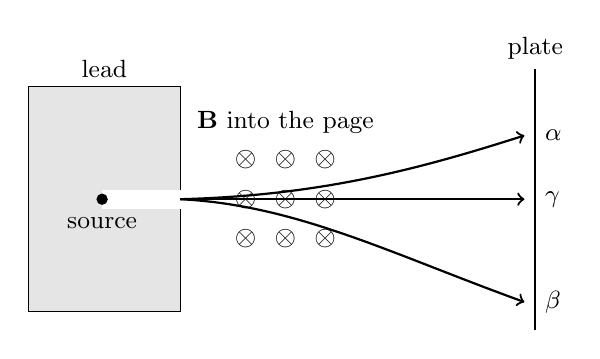
\begin{tikzpicture}[scale=0.92]
\draw[fill=gray!20] (0,-1.55) rectangle (2.1,1.55);
\draw[fill=white,draw=none] (1.02,-0.13) rectangle (2.12,0.13);
\draw[fill=black] (1.02,0) circle (0.07);
\node[below] at (1.02,-0.12) {\small source};
\node[above] at (1.05,1.55) {\small lead};
\foreach \x in {3.0,3.55,4.1}
  \foreach \y in {-0.55,0,0.55}
    \node at (\x,\y) {\(\otimes\)};
\node[above] at (3.55,0.78) {\small \(\mathbf B\) into the page};
\draw[thick] (7,-1.8) -- (7,1.8);
\node[above] at (7,1.8) {\small plate};
\draw[thick,->] (2.1,0) -- (6.85,0);
\draw[thick,->] (2.1,0) .. controls (4.0,0.05) and (5.35,0.40) .. (6.85,0.88);
\draw[thick,->] (2.1,0) .. controls (3.7,-0.08) and (5.0,-0.75) .. (6.85,-1.42);
\node[right] at (7,0.88) {\small \(\alpha\)};
\node[right] at (7,0) {\small \(\gamma\)};
\node[right] at (7,-1.42) {\small \(\beta\)};
\end{tikzpicture}\caption{횡자기장 속에서 한 방향으로 모은 방사선 빔. 중성 성분은 휘지 않고, 서로 반대 전하를 띤 성분은 휘는 정도가 서로 다르지만 반대 방향으로 휜다.}\end{figure}

세 성분에는 알파, 베타, 감마라는 이름이 붙었다. 현대적인 표현으로는,
\begin{equation}
\begin{aligned}
\beta\text{-radiation} &= \text{electrons},\\
\alpha\text{-radiation} &= \text{helium nuclei},\\
\gamma\text{-radiation} &= \text{photons}.
\end{aligned}
\end{equation}
알파 입자는 양성자 두 개와 중성자 두 개로 이루어져 있으므로 질량수가 4이다. 돌턴의 근사적인 정수 계열에서 헬륨은 수소 원자핵 질량을 단위로 네 단위인 4번에 해당했을 것이다. 베타선은 음전하를 띤 전자로, 음극선 실험을 통해 이미 알려져 있었다. 감마선은 전하를 띠지 않는다.

충분히 묽은 선원을 사용하고 개별 도달을 구분할 수 있는 검출기를 쓰면, 연속적으로 보이던 감광은 서로 떨어진 사건들의 연속으로 바뀐다. 깜빡, 깜빡, 깜빡. 베타선, 알파선, 감마선에도 같은 방법을 적용할 수 있다. 초기 장치가 정확히 그런 조건에서 작동했는지와 관계없이, 가이거 계수기는 이런 모습을 보여 준다. 각 성분은 불연속적인 다발로 도달한다. 감마선은 여전히 수수께끼다. 중성인데도 한 번에 하나씩 검출되기 때문이다. 감마선은 에너지가 매우 높은 빛이며, 플랑크와 특히 아인슈타인은 빛을 양자와 연결했다. 그러나 그 결론을 다루기 전에 빛이 파동이라는 고전적 증거를 진지하게 살펴보아야 한다.

\section{빛의 고전적 파동성}

고전적으로 빛은 연속성을 보여 주는 가장 뚜렷한 사례였다. 빛은 연속적인 파동으로 전파되는 전기장과 자기장으로 이루어진다. 뉴턴은 입자설을 지지했지만, 파동 실험들이 그 관점을 밀어냈다. 전하를 흔들면 전자기 복사가 발생한다. 거시적인 안테나는 전파, 마이크로파, 적외선, 가시광선, 자외선을 방출할 수 있다. 원자 안에서 움직이는 전하도 안테나처럼 작용한다. 방출된 복사는 사진 건판을 감광시킬 수 있다.

하나의 틈만으로도 파동의 거동을 처음 확인할 수 있다. 빛이 총알의 흐름이라면 작은 틈을 지난 뒤 선명하게 한곳에 모인 점이 생길 것으로 예상할 수 있다. 하지만 실제로는 조명이 퍼져 경계가 흐릿한 영역을 만든다. 그러나 퍼짐만으로는 결정적이지 않다. 입자가 틈의 가장자리에서 힘을 받아 휘었다고 상상할 수 있기 때문이다.

두 개의 틈을 이용하면 더 명확하게 검증할 수 있다. 서로 독립적인 두 입자 흐름은 두 개의 퍼진 자국을 만들고, 두 자국이 겹치는 곳이 가장 밝을 수도 있다. 파동은 다르게 거동한다. 한쪽 틈에서 온 마루가 다른 쪽에서 온 마루와 만나 서로 강화될 수도 있고, 마루가 골과 만나 서로 상쇄될 수도 있다. 따라서 스크린에는 밝고 어두운 띠가 번갈아 나타나며, 각 틈만 열었을 때 빛이 도달할 곳에도 어두운 곳이 생긴다.\footnote{이 도식은 강의 영상의 00:25:00부터 00:29:49까지 전개된 틈과 간섭 그림을 재구성한 것이다.}

\begin{figure}[h]\centering
\resizebox{\linewidth}{!}{%
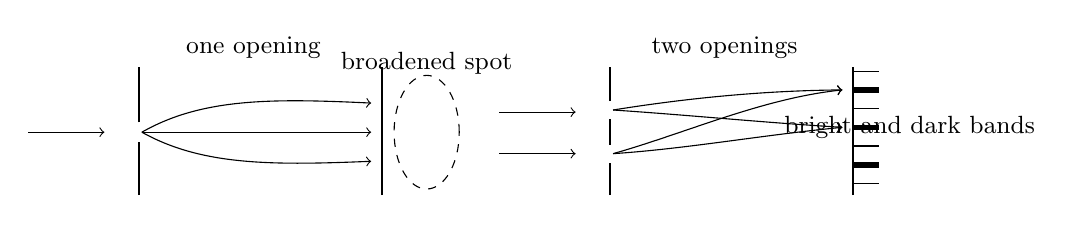
\begin{tikzpicture}[scale=0.88]
\begin{scope}
\draw[->] (-0.3,1.06) -- (0.8,1.06);
\draw[thick] (1.3,0.15) -- (1.3,0.92);
\draw[thick] (1.3,1.20) -- (1.3,2.0);
\draw[thick] (4.8,0.15) -- (4.8,2.0);
\draw[->] (1.34,1.06) .. controls (2.2,1.55) and (3.2,1.55) .. (4.65,1.48);
\draw[->] (1.34,1.06) -- (4.65,1.06);
\draw[->] (1.34,1.06) .. controls (2.2,0.58) and (3.2,0.58) .. (4.65,0.64);
\draw[dashed] (5.45,1.06) ellipse (0.47 and 0.82);
\node at (2.95,2.28) {\small one opening};
\node at (5.45,2.05) {\small broadened spot};
\end{scope}
\begin{scope}[xshift=6.8cm]
\draw[->] (-0.3,1.35) -- (0.8,1.35);
\draw[->] (-0.3,0.75) -- (0.8,0.75);
\draw[thick] (1.3,0.15) -- (1.3,0.62);
\draw[thick] (1.3,0.88) -- (1.3,1.25);
\draw[thick] (1.3,1.51) -- (1.3,2.0);
\draw[thick] (4.8,0.15) -- (4.8,2.0);
\draw[thin] (4.8,0.32) -- (5.18,0.32);
\draw[line width=2pt] (4.8,0.59) -- (5.18,0.59);
\draw[thin] (4.8,0.86) -- (5.18,0.86);
\draw[line width=2pt] (4.8,1.13) -- (5.18,1.13);
\draw[thin] (4.8,1.40) -- (5.18,1.40);
\draw[line width=2pt] (4.8,1.67) -- (5.18,1.67);
\draw[thin] (4.8,1.94) -- (5.18,1.94);
\draw[->] (1.34,0.75) .. controls (2.4,0.82) and (3.5,1.02) .. (4.65,1.13);
\draw[->] (1.34,1.38) .. controls (2.4,1.31) and (3.5,1.20) .. (4.65,1.13);
\draw[->] (1.34,0.75) .. controls (2.4,1.05) and (3.5,1.55) .. (4.65,1.67);
\draw[->] (1.34,1.38) .. controls (2.4,1.55) and (3.5,1.66) .. (4.65,1.67);
\node at (2.95,2.28) {\small two openings};
\node at (5.62,1.13) {\small bright and dark bands};
\end{scope}
\end{tikzpicture}}\caption{하나의 틈은 상이 퍼지게 하고, 두 개의 틈은 보강 간섭과 상쇄 간섭이 번갈아 나타나게 한다.}\end{figure}

물결을 떠올리면 같은 효과를 쉽게 상상할 수 있다. 손가락 두 개로 수면을 흔들면 원형 파동이 퍼져 나가며, 어떤 곳에서는 서로 강화되고 다른 곳에서는 서로 상쇄된다. 단순한 퍼짐이 아니라 간섭이 결정적인 파동의 징표다.

역사적 전개 역시 단순하지 않다. 이 도식적인 설명에서는 파동 전파를 옹호한 하위헌스가 뉴턴보다 앞에 놓이고, 토머스 영은 간섭을 입증한 인물과 연결된다. 뉴턴은 입자설을 지지했지만, 그가 직접 수행한 광학 실험 가운데 일부도 파동 간섭으로 해석할 수 있다. 후대의 간섭 실험은 빛의 파동성을 의심할 여지 없이 확립했다.

이어서 맥스웰은 무엇이 진동하는지 밝혀냈다. 빛의 파동이 한 축을 따라 전파된다면 전기장은 그 축에 수직인 횡방향이다. 자기장도 횡방향이며 전기장에 수직이다. 이 전체 패턴은 빛의 속도로 이동한다.\footnote{이 도식은 강의 영상 00:31:08에 그려진 전자기파 그림을 재구성한 것이다.}

\begin{figure}[h]\centering
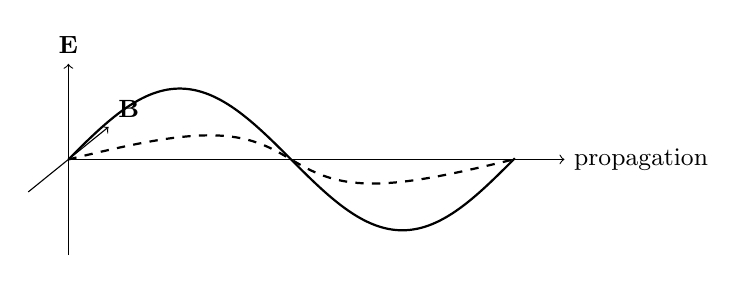
\begin{tikzpicture}[
  scale=0.9,
  x={(1cm,0cm)},
  y={(0cm,1cm)},
  z={(0.42cm,0.34cm)}
]
\draw[->] (0,0,0) -- (7,0,0) node[right] {\small propagation};
\draw[->] (0,-1.35,0) -- (0,1.35,0) node[above] {\small \(\mathbf E\)};
\draw[->] (0,0,-1.35) -- (0,0,1.35) node[above right] {\small \(\mathbf B\)};
\draw[thick,smooth,variable=\x,domain=0:6.3,samples=100]
  plot ({\x},{sin(\x r)},0);
\draw[thick,dashed,smooth,variable=\x,domain=0:6.3,samples=100]
  plot ({\x},0,{sin(\x r)});
\end{tikzpicture}\caption{전자기파에서 전기장과 자기장은 서로 수직이며, 둘 다 전파 방향에 수직이다.}\end{figure}

가시광선의 진동은 너무 빨라 전기장과 자기장의 교대 변화를 직접 따라갈 수 없다. 파장이 매우 긴 전파라면 진동은 그만큼 느려진다. 어느 경우든 같은 횡파의 기하학적 구조가 간섭을 일으킨다.

\section{파장, 주기, 진동수}

파장 \(\lambda\)은 공간상의 거리다. 진동의 한 지점에서 출발해 파동을 따라가다가 한 주기를 완전히 지난 뒤 같은 위상이 다시 나타나는 지점까지의 거리로 정의한다. 단위는 미터, 센티미터 등 길이 단위를 사용한다.

이제 한 위치에 서서 파동이 지나가는 것을 보자. 한 주기를 완전히 도는 데 필요한 시간이 주기 \(T\)이다. 가시광선의 주기는 대략 \(10^{-15}\,\mathrm{s}\) 정도로 매우 짧다. 파장이 길수록 주기는 길고, 파장이 짧을수록 주기는 짧다.

한 주기 동안 파동은 파장 하나만큼 나아가므로, 속력이 \(v\)인 파동은 다음 관계를 만족한다.
\begin{equation}
v=\frac{\lambda}{T}.
\end{equation}
물결과 음파는 각각 고유한 전파 속력을 가진다. 빛의 경우에는
\begin{equation}
c=\frac{\lambda}{T}.
\end{equation}
진동수 \(f\)는 단위 시간당 주기의 수다.
\begin{equation}
f=\frac{1}{T}.
\end{equation}
따라서
\begin{equation}
\lambda f=c.
\end{equation}
파장이나 진동수 중 하나를 알면 다른 하나도 정해진다.

\begin{figure}[h]\centering
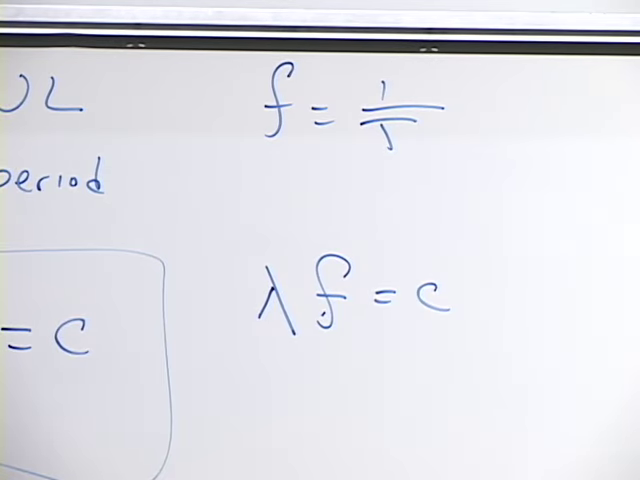
\includegraphics[width=0.68\textwidth]{lecture_01_figure_03.png}\caption{빛의 파동에서는 \(f=1/T\)이고 \(\lambda f=c\)이다.}\lectureframe{00:36:24}\end{figure}

물리학자들은 진동률을 완전한 주기의 초당 횟수 대신 초당 라디안으로 나타내는 경우가 많다. 원을 따라 등속 운동하는 상황을 생각해 보자. 어떤 점이 매초 \(f\)바퀴를 돌고, 한 바퀴가 \(2\pi\)라디안이라면 각진동수는 다음과 같다.
\begin{equation}
\omega=2\pi f,
\qquad
\frac{\omega}{2\pi}=f.
\end{equation}
지금은 이를 정의로 받아들이자. 이것이 \(2\pi\)의 인자 수를 줄여 주는지는 뒤에서 다시 살펴본다.

\(f=c/\lambda\)과 \(\omega=2\pi f\)을 결합하면 다음을 얻는다.
\begin{equation}
\omega=\frac{2\pi c}{\lambda},
\qquad
\omega\lambda=2\pi c.
\end{equation}
다른 종류의 파동에서는 \(c\) 자리에 그 파동의 전파 속력을 넣는다.

\begin{figure}[h]\centering
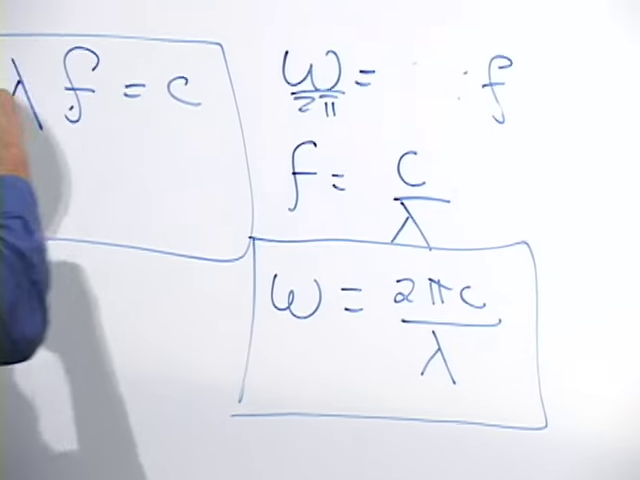
\includegraphics[width=0.68\textwidth]{lecture_01_figure_04.png}\caption{\(\omega=2\pi f\)일 때 빛의 파동은 \(\omega=2\pi c/\lambda\)을 만족한다.}\lectureframe{00:39:10}\end{figure}

전자기 복사는 연속적인 스펙트럼을 이룬다. 파장이 긴 것에서 짧은 것 순으로 배열하면 통상 다음과 같이 부른다.
\begin{equation}
\begin{aligned}
\text{radio}
&\longrightarrow \text{microwave}
\longrightarrow \text{infrared}
\longrightarrow \text{visible}\\
&\longrightarrow \text{ultraviolet}
\longrightarrow \text{X ray}
\longrightarrow \text{gamma ray}.
\end{aligned}
\end{equation}
가시광선은 이 가운데 좁은 구간만 차지한다. 각 영역의 경계는 관례에 따른 것이므로 여기서는 정확한 경계 파장이 필요하지 않다. 전파의 파장은 매우 길 수 있고, 감마선은 전자기 스펙트럼에서 파장이 가장 짧은 끝에 해당한다. 이제 어려움이 분명해졌다. 고전적으로 감마선은 연속적인 장의 파동이지만, 검출될 때는 불연속적인 깜빡임으로 나타난다.

\section{불연속적인 도달과 파동 확률}

복사의 열역학적 성질을 연구한 플랑크와 아인슈타인은 빛을 불연속적인 단위로 다루어야 한다는 결론에 이르렀다. 가상의 실험을 생각하면 그 점이 선명해지지만, 이는 실제 발견이 역사적으로 그런 경로를 따랐다는 주장이 아니다.

스크린에 빔을 비춰 보자. 보통 세기에서는 연속적으로 보이는 빛 무리가 생긴다. 빔의 일부를 가리는 감쇠기를 넣으면 빛 무리는 희미해진다. 감쇠를 거듭해서 높이면 단위 시간당 도달하는 빛의 양이 줄어든다. 그러다가 마침내 보이는 모습이 달라진다. 연속적으로 희미해진 빛 무리 대신 검출기에 고립된 사건들이 기록된다.\footnote{이 도식은 강의 영상의 00:42:32부터 00:45:42까지 전개된 감쇠 실험을 재구성한 것이다.}

\begin{figure}[h]\centering
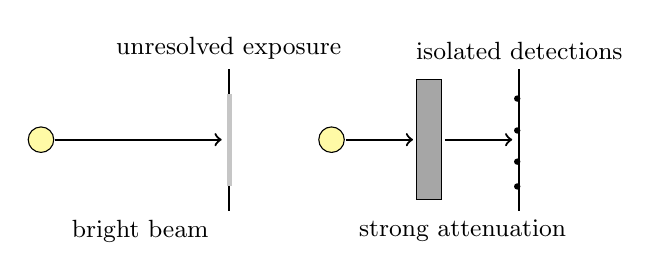
\begin{tikzpicture}[scale=0.9]
\begin{scope}
\draw[fill=yellow!35] (0,0) circle (0.18);
\draw[->,thick] (0.2,0) -- (2.55,0);
\draw[thick] (2.65,-1.0) -- (2.65,1.0);
\node[below] at (1.4,-1.0) {\small bright beam};
\end{scope}
\begin{scope}[xshift=4.1cm]
\draw[fill=yellow!35] (0,0) circle (0.18);
\draw[->,thick] (0.2,0) -- (1.15,0);
\draw[fill=gray!70] (1.2,-0.85) rectangle (1.55,0.85);
\draw[->,thick] (1.6,0) -- (2.55,0);
\draw[thick] (2.65,-1.0) -- (2.65,1.0);
\node[below] at (1.85,-1.0) {\small strong attenuation};
\end{scope}
\fill[gray!45] (2.62,-0.65) rectangle (2.70,0.65);
\foreach \y in {-0.66,-0.31,0.13,0.58}
  \fill (6.72,\y) circle (0.045);
\node[above] at (2.65,1.0) {\small unresolved exposure};
\node[above] at (6.75,1.0) {\small isolated detections};
\end{tikzpicture}\caption{점진적으로 감쇠하면 검출률이 낮아져 연속적으로 보이는 감광이 고립된 광자 사건들로 분해된다.}\end{figure}

충분히 오래 기다리면 사건들이 쌓여 원래 빛 무리와 같은 공간 분포를 이룬다. 따라서 밝게 보였던 영역은 개별 도달 사건들이 분해되지 않은 채 합쳐진 것이었다. 이 저세기 실험은 실제로 할 수 있지만, 광자 가설의 최초 동기가 된 초기 실험은 아니었다. 아인슈타인의 광자 가설은 열역학적 고려와 광전 효과에서 비롯되었다. 감쇠 실험은 그 가설의 결과를 특히 직접적으로 떠올리게 해 준다.

이제 빔 속에 두 개의 틈을 두고 광자가 한 번에 하나씩 도달할 때까지 세기를 낮추자. 검출될 때마다 국소화된 깜빡임 하나가 기록된다. 그런데 검출이 많이 쌓이면 밝고 어두운 띠를 포함한 간섭 무늬가 채워진다. 불연속적인 도달은 무작위로 일어나지만, 그 확률 분포는 파동 무늬가 예측하는 분포와 같다. 고전적인 파동은 확률을 지배하는 파동이 되었다.

그러므로 파동과 입자는 자연의 서로 다른 부분에 각각 배정된 별개의 실체가 아니다. 둘은 같은 양자 대상이 드러내는 두 가지 모습이다. 빛을 파동으로만 또는 입자로만 적절하게 설명할 수는 없다.

전자는 처음과 반대되는 놀라움을 안겨 준다. 전자는 입자로 받아들여졌고 검출기에 한 번에 하나씩 도달하지만, 서로 가까운 틈을 두면 간섭 무늬도 만든다. 전자보다 질량이 약 팔천 배 큰 알파 입자에도 같은 원리가 적용되지만, 실험은 더 어렵다. 버키볼에서도 간섭이 관측되었다. 버키볼은 탄소 원자 육십 개가 일반화된 축구공 모양에 가깝게 배열된 분자다. 볼링공에도 같은 원리가 적용될 것으로 예상되지만, 그런 실험은 현실적으로 거의 불가능하다. 바이러스나 살아 있는 세포를 대상으로 제안된 실험까지 논의를 확장할 수도 있다. 이는 점점 더 대담한 사례들이다. 파동과 입자의 설명이 어떻게 양립하는지 이해하려면 양자역학이 필요하다. 지금 할 일은 입자물리학에 필요한 광자의 성질을 추려내는 것이다.

\section{광자 에너지}

광자는 빛을 이루는 불연속적이고 더는 나눌 수 없는 요소다. 빛은 에너지를 운반한다---햇빛은 흡수하는 물체를 데운다---따라서 광자 하나하나가 에너지를 가져야 한다. 단색파는 파장과 각진동수가 정해져 있으며, 그 파동의 광자는 모두 다음 에너지를 가진다.
\begin{equation}
E_\gamma=\hbar\omega.
\end{equation}
연속적인 파동을 작은 점들이 모인 기계적 집합으로 그려 보려는 것은 오해를 부른다. 분명한 것은 실험에서 관측되는 조합이다. 국소화된 검출 사건이 파동이 결정하는 분포에 따라 일어나고, 에너지는 나눌 수 없는 단위로 도달한다.

\begin{equation}
\omega=\frac{2\pi c}{\lambda},
\end{equation}이므로
파장이 짧을수록 각진동수가 크고 따라서 광자 하나의 에너지도 크다.
\begin{equation}
\lambda\downarrow
\quad\Longrightarrow\quad
\omega\uparrow
\quad\Longrightarrow\quad
E_\gamma\uparrow.
\end{equation}
전파 광자 하나의 에너지는 매우 작다. 하지만 전파 빔에는 광자가 아주 많이 들어 있을 수 있으므로, 빔 전체는 막대한 에너지를 운반할 수 있다. \(n\)개의 광자가 들어 있는 단색 펄스라면,
\begin{equation}
E_{\text{pulse}}=n\hbar\omega,
\qquad
n=0,1,2,\ldots.
\end{equation}
총에너지는 클 수 있지만, 여전히 광자 하나의 에너지에 정수배를 곱한 값이다.

이 관계는 앞으로 논의의 방향을 결정할 실용적인 질문으로 이어진다. 더 작은 것을 보려면 왜 점점 더 큰 기계를 만들어야 하는가? 작은 물체를 보는 데 작은 기계를 쓰면 안 되는가? 답의 전반부는 이미 나왔다. 더 작은 구조를 분해해 보려면 더 짧은 파장이 필요하고, 파장이 짧은 양자는 더 큰 에너지를 가진다.

\section{정지 에너지와 불변 질량}

입자물리학은 양자역학과 상대성이론을 결합한다. 광자 관계식 \(E_\gamma=\hbar\omega\)은 양자론 쪽을 제공하고, 상대성이론에서 대응하는 기본 사실은 다음과 같다.
\begin{equation}
E_{\mathrm{rest}}=mc^2.
\end{equation}
이때의 한정은 중요하다. 오래된 설명에서는 \emph{정지 질량}과 속도에 따라 달라지는 \emph{운동 질량}을 구별했다. 현대 용어에서 \emph{질량}은 물체의 불변 질량을 뜻한다. 운동은 에너지를 바꾸지만 질량은 바꾸지 않는다. 어떤 상태로 운동하든 전자의 질량은 모두 같지만, 전자가 가속되면 에너지는 증가한다. 따라서 이 형태의 \(E=mc^2\)은 물체 전체가 정지해 있는 기준계에서 질량을 가진 물체의 에너지를 나타낸다.

물체가 정지해 있어도 내부 구성 요소까지 정지해 있을 필요는 없다. 기체 상자는 저울 위에서 정지해 있어도 분자들은 모든 방향으로 빠르게 움직일 수 있다. 이러한 내부 운동의 에너지는 상자 전체의 정지 에너지에 포함된다. 차가운 상자에서 시작해 질량을 측정한 뒤, 상자 자체는 정지한 채 열에너지를 더해 보자. 정지 질량은 다음만큼 변한다.
\begin{equation}
\Delta m=\frac{\Delta E_{\mathrm{internal}}}{c^2}.
\end{equation}
질량이 늘어나면 무게와 관성도 커진다. 보통 상자에서는 온도를 크게 높여도 일반적인 저울로 그 효과를 알아차리기에는 너무 작다. 효과가 작다고 해서 원리가 달라지는 것은 아니다.

더 분명한 예로 전자와 양전자를 들 수 있다. 두 입자의 질량은 정확히 같고 전하는 서로 반대다. 처음에 정지해 있던 두 입자가 소멸하면 광자들이 에너지를 가져간다.
\begin{equation}
e^-+e^+\longrightarrow \text{photons}.
\end{equation}
초기 에너지는
\begin{equation}
E_{\mathrm{initial}}=2m_e c^2,
\end{equation}
이며, 그 에너지는 사라질 수 없다. 쌍 하나가 내놓는 에너지는 아주 적으므로 커피 한 잔을 데우려 해도 엄청나게 많은 쌍이 필요하다. 하지만 개별 소멸 사건은 변환을 직접 보여 준다.

따라서 정지한 물체의 질량과 에너지는 단위만 다르게 표현한 같은 물리량이다. \(c^2\)은 관습적인 질량 단위와 에너지 단위 사이의 환산 인자이며, 수를 미터에서 센티미터로 바꾸는 환산 인자와 비슷하다.

\begin{classroomqa}\lecturetimestamp{01:04:39}\audiencequestion{질량이 방출된 에너지로 바뀌려면 어떤 메커니즘이 필요한가?}\lecturerresponse{그렇다. 물리적 메커니즘이 필요하지만, 보존 법칙만으로도 그 결과에 이미 제약이 주어진다. 미시적인 소멸 메커니즘을 설명하기 전에도, 초기 전자--양전자 에너지는 어딘가에서 다시 나타나야 한다. 따라서 상호작용을 자세히 설명하지 않아도 에너지 보존으로 답의 중요한 부분을 알아낼 수 있다.}\end{classroomqa}

\section{차원과 단위의 선택}

SI 단위계에서 빛의 속력은 매우 큰 수로, 플랑크 상수는 매우 작은 수로 나타난다. 후자가 작다는 점은 광자 관계식만 보아도 알 수 있다. 가시광선의 각진동수는 엄청나게 큰 반면 광자 하나의 에너지는 매우 작으므로, 이 단위계에서 \(E_\gamma=\hbar\omega\)가 성립하려면 \(\hbar\)의 수치가 작아야 한다. 크기 차수만 나타내면 다음과 같다.
\begin{equation}
c\sim 10^8\ \mathrm{m\,s^{-1}},
\qquad
\hbar\sim 10^{-34}\ \mathrm{J\,s}.
\end{equation}
\editorialnote{칠판의 마지막 자리 숫자가 흐릿하므로 강의에서 제시한 크기 차수만 유지했다.}
단위는 필수다. 두 상수 모두 단순한 소수가 아니다. 에너지의 차원은
\begin{equation}
[E]=M L^2 T^{-2},
\end{equation}
이며, \(E_\gamma=\hbar\omega\)와 \([\omega]=T^{-1}\)를 고려하면 플랑크 상수의 차원은 다음과 같다.
\begin{equation}
[\hbar]=[E]T=M L^2 T^{-1}.
\end{equation}

\(c\)이 크고 \(\hbar\)가 작다고 말하는 것 자체가 이미 단위 선택을 전제로 한다. 속력을 시간당 피트로 재면 초당 미터로 잴 때와 \(c\)의 수치가 다르다. 광년/년이나 광초/초 단위로 나타내면 빛의 속력은 1이다. 질량, 길이, 시간 단위를 서로 맞게 선택하면 \(\hbar=1\)로 둘 수도 있다.

익숙한 단위계는 자연이 특별히 정해 둔 특성이 아니라 물려받은 관례다. 마일에는 5280피트가 들어 있고, 스톤은 14파운드이며, 말의 키는 핸드 단위로 재고, 동력은 마력으로 나타낼 수 있다. 미터법 단위는 더 체계적이지만, 그 척도 역시 인간이 선택한 것이다. 기초 물리학에는 미터, 초, 킬로그램을 특별히 지목하는 요소가 없다.

길이, 시간, 질량은 서로 독립적인 세 가지 기본 단위 선택을 이룬다.
\begin{equation}
L,\qquad T,\qquad M.
\end{equation}
다른 역학 단위는 이들로부터 만들 수 있다. 어떤 선택이 유용한지는 문제에 따라 달라진다. 천체물리학에서는 태양 질량이 편리하고, 핵물리학에서는 양성자 질량이 편리할 수 있다. 상대론적 천문학 공식은 광년과 년을 쓰면 간결해진다. 서로 독립적인 선택지가 세 가지이므로 차원이 독립적인 상수 세 개에 편리한 수치를 부여할 수 있다. 천체물리학, 원자물리학, 입자물리학은 서로 다른 선택을 해도 된다.

입자물리학에서는 다음 두 관례가 특히 유용하다.
\begin{equation}
c=1,
\qquad
\hbar=1.
\end{equation}
남은 단위에 대해서는 이에 필적할 만한 특별한 입자 질량이 없다. 양성자 질량, 힉스 보손 질량, 뮤온 질량을 1로 정할 수는 있지만, 이는 수많은 입자 가운데 하나만 특별히 취급하는 것일 뿐이다.

그렇다면 왜 \(c\)와 \(\hbar\)를 선택할까? 첫 번째 답으로는 이 값들이 여러 방정식에 나타난다는 점을 들 수 있다. 하지만 자주 등장한다는 것만으로는 충분하지 않다. 양성자 질량도 여러 방정식에 나타나며, 양성자의 크기도 마찬가지다. \(c\)와 \(\hbar\)를 구별해 주는 것은 보편성이다.

상수 \(c\)와 \(\hbar\)는 서로 다른 방식으로 보편적이다. 속력 \(c\)는 모든 물리적 대상에 제약을 가한다. 질량이 있는 물체는 이 속력에 가까워질 수 있지만, 이를 넘어서도록 가속될 수는 없다. 플랑크 상수는 다음과 같은 크기 차수의 불확정성 관계를 통해 모든 양자 대상에 제약을 가한다.
\begin{equation}
\Delta x\,\Delta p\gtrsim\hbar.
\end{equation}
두 진술 모두 특정 입자종을 따로 지정하지 않는다. 이러한 보편성 때문에 \(c=1\)와 \(\hbar=1\)를 자연스러운 관례로 삼을 수 있다.

양성자에는 이에 견줄 만한 보편적인 척도가 없다. 양성자는 많은 대상 중 하나일 뿐이다. 양성자 질량을 1로 정해도 루비듐 원자 질량을 1로 정하는 것보다 더 근본적인 의미는 없다. 전자, 힉스 보손, 뮤온을 기준으로 삼아도 같은 문제가 생긴다.

전하에서도 또 다른 보편적 물리량을 찾을 수 있을 듯하지만, \(c\)와 \(\hbar\)를 표준화하고 나면 물리적으로 중요한 전자기 결합은 무차원이다. 단위 선택으로 전자기 방정식에서 차원을 가진 상수들의 위치를 바꿀 수는 있지만, 진정한 무차원 결합의 값은 바꿀 수 없다.

중력은 차원을 가진 보편 상수를 제공한다. 뉴턴의 표현에서 두 질량 사이 힘의 크기는 다음과 같다.
\begin{equation}
F=G\frac{m_1m_2}{r^2}.
\end{equation}
모든 질량은 중력으로 상호작용하지만, 전기적으로 중성인 물체는 전기력에 참여하지 않을 수 있다. 따라서 \(G\)는 필요한 보편성을 갖는다. 그럼에도 현재 논의하는 계산에서 알려진 기본 입자 사이의 중력은 무시할 수 있으므로, 보통의 입자물리학에서 이를 실용적인 단위 기준으로 삼기는 어렵다.

\begin{classroomqa}
\lecturetimestamp{01:20:34}
\audiencequestion{\(G\)을 그저 무시해도 되는가? 매우 높은 에너지에서는 기본 입자가 여기서 가정한 방식대로 고전 중력에 따르지 않을 수도 있다.}
\lecturerresponse{개별 입자는 실제로 지구의 중력장에 반응한다. 입자 하나도 그 장 안에서 낙하한다. 한 기본 입자가 다른 기본 입자에 미치는 중력의 영향은 직접 측정된 적이 없으므로, 그 수준에서는 보편성 가정에 의문을 제기할 수 있다. \(G\)을 제외하는 직접적인 이유는 절대적인 원칙이 아니라 실용성에 있다. 중력은 일반적인 입자물리학 실험과 방정식에 무시해도 될 만큼만 기여한다.}
\end{classroomqa}

\begin{classroomqa}
\lecturetimestamp{01:22:01}
\audiencequestion{중력 대신 전자기 상호작용을 세 번째 단위 설정 규약으로 사용할 수 있을까?}
\lecturerresponse{그렇다. 전하 또는 쿨롱 법칙에 등장하는 상수를 정규화하는 전자기 단위계를 선택할 수 있다. 실제로 그런 규약을 사용한다. 전자는 서로 끌어당기는 것이 아니라 밀어내지만, 이 부호가 그런 선택을 막지는 않는다. 여기서는 단지 그 규약을 채택하지 않았을 뿐이다.}
\end{classroomqa}

\begin{classroomqa}
\lecturetimestamp{01:23:06}
\audiencequestion{\(c\)과 \(\hbar\)를 1로 두면 전하는 무차원인가?}
\lecturerresponse{그렇다. 전하의 제곱과 관련된 무차원 척도는 대략 \(1/137\)이다. 정확한 규약과 그 수의 의미는 나중에 다뤄도 된다. 여기서 중요한 점은 그 값이 무차원이라는 것이다.}
\end{classroomqa}

\begin{classroomqa}
\lecturetimestamp{01:23:37}
\audiencequestion{쿨롱 상수를 세 번째로 1로 둘 상수로 선택할 수 있을까?}
\lecturerresponse{그 상수를 전자기 단위 규약에 흡수할 수는 있다. 하지만 단위를 바꾸어도 무차원 결합 상수 \(1/137\)는 달라지지 않으므로, 그 선택으로 결합 상수를 1로 만들 수는 없다. 여기서 그 규약을 채택하는 데 특별한 이점이 있다고 주장하는 것은 아니다.}
\end{classroomqa}

\section{자연 단위계의 방정식과 기준계}

\(c=1\)를 쓰면 질량이 있는 물체의 정지 에너지 관계는 다음과 같이 된다.
\begin{equation}
E_{\mathrm{rest}}=m.
\end{equation}
\(\hbar=1\)를 쓰면 광자 관계는 다음과 같이 된다.
\begin{equation}
E_\gamma=\omega.
\end{equation}
일반적인 단위계에서 수치의 크기가 필요할 때는 언제든 상수들을 다시 넣을 수 있다.

\begin{figure}[h]
\centering
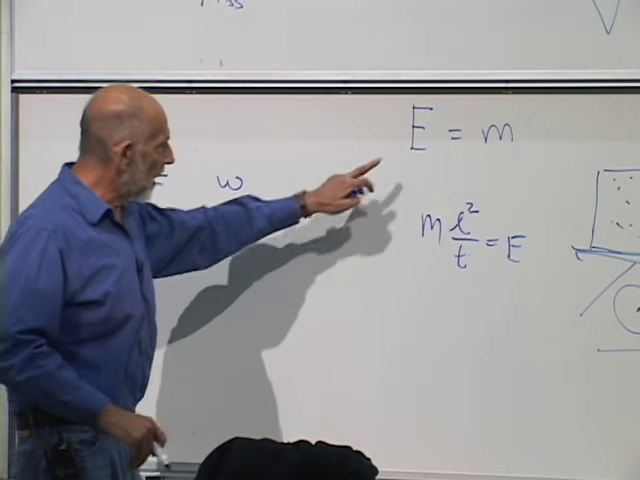
\includegraphics[width=0.72\textwidth]{lecture_01_figure_05.png}
\caption{\(c=1\)인 단위계에서 정지한 질량체의 정지 에너지는 \(E=m\)이다.}
\lectureframe{01:25:40}
\end{figure}

이 식들은 비슷해 보이지만 의미는 서로 다르다. \(E_{\mathrm{rest}}=m\)에서 \(E\)는 질량체의 정지 에너지다. 광자는 질량이 없고 정지 상태로 만들 수도 없으므로, 광자의 에너지는 정지 에너지가 아니다. 관계식 \(E_\gamma=\omega\)는 운동하는 질량 없는 양자의 에너지를 나타낸다.

\begin{classroomqa}
\lecturetimestamp{01:26:07}
\audiencequestion{정지는 언제나 어떤 대상에 대한 상대적인 상태이고 실험실 자체도 절대적으로 정지해 있지 않은데, \emph{정지}란 무슨 뜻인가?}
\lecturerresponse{정지는 선택한 기준계에 대해 정의된다. 컵이 실험실에 대해 정지해 있다면, 그 실험실 기준계에서 컵의 에너지는 \(c=1\)일 때 질량과 같으며, 전체 운동 에너지 항은 없다. 컵 곁을 지나가는 다른 관측자는 컵에 운동 에너지도 있다고 본다. 관측자마다 같은 물체나 광자에 서로 다른 에너지를 부여하는 것이 일반적이다. 에너지는 기준계에 따라 달라지며, 절대 정지를 주장할 필요는 없다.}
\end{classroomqa}

이제 각진동수 규약을 다시 살펴볼 수 있다. \(E_\gamma=\hbar\omega\)라고 쓰면 간결하지만, 앞서 \(\omega=2\pi f\)에는 \(2\pi\) 인자가 들어갔다.

\begin{classroomqa}
\lecturetimestamp{01:28:13}
\audiencequestion{초당 완전한 주기의 수라는 겉보기에 더 간단한 수 대신, 초당 라디안으로 측정하는 각진동수 \(\omega\)를 사용하는 이유는 무엇인가?}
\lecturerresponse{이 선택에는 역사적인 이유도 일부 있지만, 수학적 대답은 즉각적이라기보다 실용적인 것이다. 여기서 제시할 대답은 잠정적이다. 관련 방정식을 \(f\)를 사용해 한 번, \(\omega\)를 사용해 한 번 써 보고, 어느 규약에서 \(2\pi\) 인자가 더 적게 남는지 살펴보면 된다. 어느 쪽을 택해도 \(2\pi\) 인자가 모든 곳에서 사라지게 할 수는 없다. 복소 지수 표기법과의 연관 가능성도 제안되었지만, 여기서는 더 다루지 않는다.}
\end{classroomqa}

\begin{classroomqa}
\lecturetimestamp{01:29:51}
\audiencequestion{두 입자를 가속해 서로 간의 중력 상호작용이 중요해질 때까지 에너지를 높일 수 있을까?}
\lecturerresponse{원리적으로는 가능하다. 그러나 현재의 가속기는 실제로 그런 영역에 한참 못 미친다. 또한 답은 입자를 무엇으로 뜻하느냐에 달려 있다. 거시적인 중력체는 여기서 다루는 기본 입자와는 다른 경우다.}
\end{classroomqa}

\begin{classroomqa}
\lecturetimestamp{01:30:27}
\audiencequestion{양전자의 원천으로 무엇을 이용할 수 있는가?}
\lecturerresponse{고에너지 충돌로 양전자를 생성할 수 있다. 일부 핵 과정과 붕괴에서도 양전자가 생성된다.}
\end{classroomqa}

\begin{classroomqa}
\lecturetimestamp{01:30:53}
\audiencequestion{플랑크 시간과 플랑크 거리가 여기서 사용하는 자연 단위인가?}
\lecturerresponse{아니다. 플랑크 단위는 \(G\), \(c\), \(\hbar\)를 모두 1로 둘 때 얻어진다. 그때의 플랑크 길이는 일반적인 입자물리학의 길이 척도보다 훨씬 작으므로 여기서는 측정 기준으로 쓰기 불편하다. 중력과 양자역학, 상대론이 모두 함께 중요해지는 블랙홀 물리학, 우주론 또는 양자중력에서는 이런 단위가 자연스럽다. 중력을 무시할 수 있을 때는 \(c\)와 \(\hbar\)만 1로 두는 편이 더 유용하다.}
\end{classroomqa}

\section{운동량, 빛, 그리고 분해능}

다음 기본 개념은 운동량이다. 정지한 물체는 운동량이 없지만, 영이 아닌 정지 에너지 \(mc^2\)를 가진다. 물체가 움직이면 일반적으로 운동량을 가진다. 에너지가 보존되듯 운동량도 충돌에서 보존된다. 두 물체가 충돌할 때 충돌 전후의 전체 벡터 운동량은 같다. 보존 법칙의 제약을 받는 것은 무엇이든 특별히 주목할 만하다.

운동량은 벡터이며 운동 방향을 가리킨다. 비상대론적 물체의 경우,
\begin{equation}
\mathbf p=m\mathbf v.
\end{equation}
이는 일반적인 상대론적 공식이 아니며, 빛에 직접 적용할 수 없다.

그렇지만 빛은 에너지뿐 아니라 운동량도 가진다. 보통의 빛이 만들어 내는 미는 힘은 너무 작아 운동량을 알아차리기 어렵지만, 강한 레이저 펄스는 상당한 충격량을 전달할 수 있다. 예를 들어 리버모어의 대형 레이저는 복사가 운반하는 운동량으로 물질을 안쪽으로 밀어 넣을 수 있다.

광선이 거의 한 축을 따라 진행할 만큼 충분히 평행한 펄스를 생각해 보자. 실제 빔에는 어느 정도 각도 퍼짐이 있어 빔의 일부가 조금씩 다른 방향으로 진행할 수 있지만, 이상적으로 평행한 빔의 운동량은 빔을 따라가며 그 크기는 다음과 같다.
\begin{equation}
p=\frac{E}{c},
\qquad\text{or equivalently}\qquad
E=cp.
\end{equation}
여기서는 이 관계를 증명하기보다는 상대론적 사실로 받아들인다. 다음 차원 검사는 그 단위가 보통의 운동량 단위와 일치하는지만 확인한다.
\begin{equation}
\left[\frac{E}{c}\right]
=
\frac{M L^2 T^{-2}}{L T^{-1}}
=
M L T^{-1}
=
[m v]
=
[p].
\end{equation}
이 차원 비교는 빛에 정지 질량을 부여하지 않는다. 광자의 질량은 0이다. 광자는 에너지를 가지고 \(c\)로 움직이기 때문에 운동량을 가진다.

\(\mathbf p\)의 방향은 전파 방향이다. 분모에 \(c\)가 들어가므로 그 크기를 감지하기는 대개 어렵다. 빔은 물질을 가열하거나 증발시켜 그 에너지를 쉽게 드러낼 수 있지만, 빔이 가하는 역학적 압력은 훨씬 작다. 그러나 세기를 충분히 높이면 그 압력도 커질 수 있다.

광자 하나에 대해서는
\begin{align}
p_\gamma
&=\frac{E_\gamma}{c}\\
&=\frac{\hbar\omega}{c}.
\end{align}
이를 파장으로 나타내려면 파동 관계식을 주의 깊게 다시 살펴보자. 다음 관계에서
\begin{equation}
f\lambda=c,
\qquad
\omega=2\pi f,
\end{equation}
올바른 관계는 다음과 같다.
\begin{equation}
\omega\lambda=2\pi c,
\qquad
\omega=\frac{2\pi c}{\lambda}.
\end{equation}
정의를 써서 확인하지 않으면 \(2\pi\) 인자를 뒤집기 쉽다. \(f\lambda=c\)와 \(f=\omega/(2\pi)\)에서 다시 시작하면 문제가 명확해진다.
\begin{equation}
\frac{\omega}{2\pi}\lambda=c
\quad\Longrightarrow\quad
\omega\lambda=2\pi c.
\end{equation}
이제 대입하면 다음을 얻는다.
\begin{align}
p_\gamma
&=\frac{\hbar}{c}\frac{2\pi c}{\lambda}\\
&=\frac{2\pi\hbar}{\lambda}\\
&=\frac{h}{\lambda}.
\end{align}

\begin{classroomqa}
\lecturetimestamp{01:42:38}
\audiencequestion{\(2\pi\hbar\)는 \(h\)와 같은가?}
\lecturerresponse{그렇다. 정의에 따라 \(h=2\pi\hbar\)이므로, \(p_\gamma=2\pi\hbar/\lambda\)는 \(p_\gamma=h/\lambda\)와 같다. 어떤 진동수 규약을 선택해도 \(2\pi\) 인자는 어디엔가 다시 나타난다.}
\end{classroomqa}

파장이 짧을수록 광자의 운동량은 크다. 전파 광자는 파장이 매우 길고 운동량이 아주 작다. 감마선 광자는 파장이 매우 짧아 훨씬 큰 충격을 준다. 광자 하나가 주는 거시적인 충격량은 여전히 작지만, 전파 광자에 비하면 운동량이 훨씬 크다. \(E_\gamma=cp_\gamma\)이므로 에너지도 더 크다.

이 관계는 더 작은 물체를 관찰할수록 더 큰 장치가 필요한 이유를 설명한다. 사람 머리보다 훨씬 긴 파장의 사진으로는 흐릿한 모습만 볼 수 있다. 얼굴의 특징을 구분하려면 파장이 머리보다 짧아야 한다. 머리카락 하나를 분해하려면 파장이 머리카락의 굵기와 비슷하거나 그보다 작아야 한다. 원자의 구조를 분해하려면 탐침 파장이 원자보다 크지 않아야 한다.
\begin{equation}
\lambda_{\mathrm{probe}}\lesssim
\text{size of the structure to be resolved}.
\end{equation}
따라서 더 작은 구조를 관찰하려면 더 짧은 파장이 필요하고, 더 짧은 파장에는 더 큰 운동량과 에너지가 필요하다. 탐침이 반드시 광자여야 하는 것은 아니다. 다른 종류의 고에너지 입자에도 파장과 운동량 사이의 같은 양자적 관계가 성립한다. 그런 입자를 만들려면 입자 하나하나에 점점 더 많은 에너지를 전달하는 가속기가 필요하다. \(p_\gamma=h/\lambda\)와 \(E_\gamma=\hbar\omega\)의 관계가 이 논리를 뒷받침한다. 탐침 에너지를 높이면 운동량은 커지고 파장은 짧아진다.

대략 한 세기 동안 입자물리학에서 반복되어 온 양상은 이렇다. 에너지가 높아질수록 운동량이 커지고, 파장이 짧아지며, 공간 분해능이 높아진다.

\begin{classroomqa}
\lecturetimestamp{01:46:57}
\audiencequestion{파장에 이론적인 하한이 있을까?}
\lecturerresponse{그럴 가능성이 있다. 플랑크 길이 부근에서 새로운 현상이 나타날 것으로 예상되지만, 이는 잠정적인 답이다. 공간 분해능이 그곳에서 더는 높아지지 않는다고 해도, 그 척도는 LHC에서 탐사하는 거리보다 약 17자릿수나 작다. 따라서 현재 실험은 그 규모에 훨씬 못 미친다.}
\end{classroomqa}

같은 논리를 따라가면 가속기의 규모와 그 가속기로 분해할 수 있는 규모 사이에 대략적인 관계가 있음을 알 수 있다.

\begin{classroomqa}
\lecturetimestamp{01:48:02}
\audiencequestion{파장 또는 분해하려는 대상의 크기는 가속기의 크기에 대략 반비례하는가?}
\lecturerresponse{대략 그렇다. 다만 입자를 가속하는 최대 전기장과 입자의 진행 방향을 유도하는 자기장이 장치가 제공할 수 있는 범위 안에서 고정되어 있다고 가정해야 한다. 가속 기울기는 단위 길이당 에너지 증가량이다. 길이가 \(L\)이고 가속 기울기 \(\mathcal G\)가 대략 일정한 선형 가속기의 경우,
\[
E_{\mathrm{beam}}\sim \mathcal G L.
\]
초상대론적 에너지에서는 분해할 수 있는 파장이 에너지에 반비례하므로, 선형 가속기의 길이를 늘리면 분해능은 대략 그 역비만큼 높아진다. 이는 정확한 법칙이 아니라 경험적 규모 추정이다. 원형 가속기에서는 같은 장치를 여러 차례 통과시킬 수 있지만, 휘어지는 동안 가속된 전하가 복사를 방출해 에너지를 잃는다.}
\end{classroomqa}

\begin{classroomqa}
\lecturetimestamp{01:49:47}
\audiencequestion{플랑크 길이에 도달하려면 가속기의 크기가 어느 정도여야 하는가?}
\lecturerresponse{이 대략적인 규모 추정에 따르면 CERN의 가속기보다 약 17자릿수 더 길어야 한다. 우주의 크기까지는 아니지만, 대략 은하 규모다.}
\end{classroomqa}

\begin{classroomqa}
\lecturetimestamp{01:50:09}
\audiencequestion{최고 에너지 우주선의 에너지는 충돌기 에너지와 어떻게 비교되는가?}
\lecturerresponse{개별 우주선의 실험실 에너지는 훨씬 클 수 있다. 수치로 비교하기 위해 실험실 에너지가 대략 \(10^{21}\,\mathrm{eV}=10^{12}\,\mathrm{GeV}\)인 극단적인 우주선을 생각해 보자. 그러나 우주선은 실험실에서 정지해 있는 표적을 때리는 반면, 충돌기에서는 에너지가 큰 두 빔을 정면으로 충돌시킨다. 더 중요한 점은 유용한 실험에는 입자속, 즉 많은 입자와 잘 제어된 많은 충돌이 필요하다는 것이다. 우주선 하나는 관련 표적을 빗나갈 수도 있고, 무엇을 추론하기 어려운 사건을 만들 수도 있다. 유용한 은하 규모 가속기를 가동하는 데 필요한 전력을 석유 소비량으로 바꾸어 과장되게 추산한 결과, 초당 약 100조 배럴의 석유가 필요하다는 값이 제시되었다. 이 추산의 요지는 충분한 충돌 통계를 확보하는 일이 가속기의 길이만큼이나 심각한 장애물임을 보이는 데 있다.}
\end{classroomqa}

\editorialnote{석유 환산 추산은 원문에서 일관되지 않는다. 처음 제시한 뒤 초당 약 \(10^{14}\)배럴이라고 반복하지만, 나중에 다시 언급할 때는 초당 \(10^{11}\)배럴이라고 한다. 두 규모를 모두 남겨 두고 임의로 조정하지 않았다.}

이 거리 척도는 단지 형식적인 것이 아니라 실제로 존재한다. 실질적인 난제는 은하 규모의 가속기를 만들고 그 막대한 전력을 공급하지 않고도 그런 척도를 어떻게 탐사할 것인가이다.

\begin{classroomqa}
\lecturetimestamp{01:52:55}
\audiencequestion{LHC의 에너지는 \(10^{12}\,\mathrm{GeV}\) 에너지의 우주선과 어떻게 비교해야 하는가?}
\lecturerresponse{실험실에서 에너지가 \(E_{\mathrm{lab}}\)인 초상대론적 입사 입자가 질량 \(m_{\mathrm{target}}\)인 고정 표적을 때릴 때, 질량중심 에너지는 매개변수적으로 다음과 같이 주어진다.
\[
E_{\mathrm{cm}}\simeq
\sqrt{2m_{\mathrm{target}}c^2E_{\mathrm{lab}}}.
\]
\editorialnote{고정 표적 식을 표시해, 이 문답에서 언급한 제곱근에 비례하는 관계를 명시했다.}
표적 질량을 고정하면 유용한 충돌 에너지는 입사 입자 에너지의 제곱근만큼만 증가한다. 따라서 \(10^{12}\,\mathrm{GeV}\) 에너지의 우주선은 규모 추정상 서로 반대 방향으로 진행하는 빔 각각의 에너지가 \(10^6\,\mathrm{GeV}\) 정도인 경우에 해당하며, 각 빔이 \(10^{12}\,\mathrm{GeV}\)인 경우에 해당하지 않는다. 우주선의 에너지는 여전히 지상 충돌기의 에너지를 넘어설 수 있지만, 우주선의 속이 매우 낮아 체계적이고 통제된 실험에는 적합하지 않다.}
\end{classroomqa}